\TODO{
    Here describe plugin for SonarQube.
    In introduction we mentioned groups that we think the tool might be used for.
    So here we provide our ideas how each group can be helped with our tool,
    provide screenshots or other artifacts that might help our points.

    Describe how queries are transformed into sonarqube implementation
    Describe how we tested the tool (We have X test cases and code coverage was Y percent etc).

    Also describe the results of developing the bulk analyzer, provide simple
    instructions on how to run this tool, provide output from help command, which
    will show input parameters and basic instruction on how to run.
}

\subsubsection{Implementation}\label{subsec:implementation}

\TODO {
Describe implementation of the tool here.
How many lines of code?
Classes?
Provide an architechtural diagram.
Purpose of this section is to give an overview to the reader who would not check the repository to understand
how much work was done.
Also mention that this tool is open source and provide link to the repository.
}

\TODO{
Count how many classes there are in implementation
}

As the result of development we created a plugin that is able to detect 30 code smells.
The resulting implementation contains $X$ classes and 6476 lines of Scala code.
This number includes tests but does not include test resources (Java files that were
used to test code smell detection).

\TODO{
Add figure of architecture and flow
}

The basic flow of the plugin operation can be seen on figure $X$.
Firstly, we have to register our plugin inside a SonarQube instance.
Secondly, we have to load our rules and descriptions of the rules into the instance of SonarQube.
Finally, the user can create a new profile with our rules or add the rules to an existing
profile and then run the analysis using the rules that we provide inside our plugin.

As mentioned previously in section~\ref{subsec:sonarqube-plugin-development}, the plugin itself operates on the Java
AST\@.
As an example, we provided an implementation of \say{Complex class} rule which can be seen in figure~\ref{complex_class_implementation}.
This code smell inspects all class nodes which are found in the AST, calculates the complexity of all methods
in the class and reports an issue if the complexity of the class is greater than configured threshold.

\begin{figure} [htb]
    \lstset{language=Scala}
    \begin{lstlisting}
@Rule(key = "ComplexClass")
class ComplexClass
    extends JavaRule
    with ComplexityAccessor
    with ContextReporter {

        private var context: JavaFileScannerContext = _

        private var veryHighClassComplexity: Double = _

        override def scanFile(
        javaFileScannerContext: JavaFileScannerContext): Unit = {
            this.context = javaFileScannerContext

            veryHighClassComplexity = config
            .flatMap(
            _.getDouble(
            ConfigurationProperties.COMPLEX_CLASS_VERY_HIGH_COMPLEXITY.key))
            .orElse(
            ConfigurationProperties.COMPLEX_CLASS_VERY_HIGH_COMPLEXITY.defaultValue.toDouble)

            scan(context.getTree)
        }

        override def scannerContext: JavaFileScannerContext = context

        override def visitClass(tree: ClassTree): Unit = {
            val classComplexity = tree.members.asScala
            .filter(_.is(Kind.METHOD))
            .map(_.asInstanceOf[MethodTree])
            .map(complexity)
            .sum

            report(
            s"Complex class: class complexity $classComplexity is higher than configured: $veryHighClassComplexity",
            tree,
            classComplexity >= veryHighClassComplexity
            )

            super.visitClass(tree)
        }
    }
    \end{lstlisting}
    \caption{Implementation of "Complex class" rule.}
    \label{complex_class_implementation}
\end{figure}

\FloatBarrier

The high level architecture of the plugin can be seen on figure~\ref{architecture_diagram}.
The plugin initialization is started when SonarQube loads the plugin into memory.
When the plugin is loaded, the plugin registers its extensions and delegates all of the
further work to the extensions.
Currently there are 2 extensions, rules registrar (\verb|SonarAcademicRulesRegistrar|) and
sensor (\verb|SonarAcademicSensor|).


The purpose rules registrar is to load all of the rules, their descriptions and then register
those rules with the SonarQube so that the rules are could be enabled or disabled by the
user in the SonarQube user interface and further be used in the analysis.


The sensor acts as a bridge between SonarQube and rules which require context during their runtime.
The idea is that sensor receives a whole project as an input, as opposed to single files which is the case for the
regular rules, and then feeds individual files to the sensor rules.
The difference between regular rules and sensor rules is explained in section~\ref{subsubsec:translating-queries}.

After the plugin has been loaded, SonarQube delegates analysis of single files to the rules.
For sensor rules, SonarQube delegates the whole project and then the sensor performs analysis of single
files for all sensor rules.

\begin{figure}[ht]
    \begin{center}
        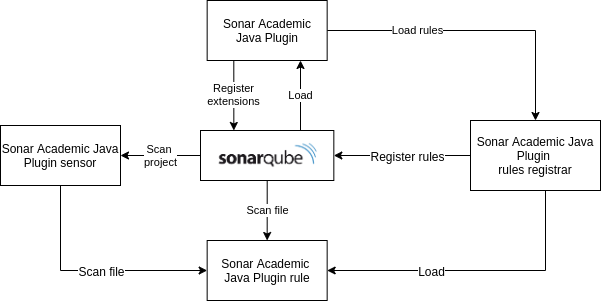
\includegraphics[scale=0.7]{figures/architecture_diagram.png}
        \caption{High level architecture of Sonar Academic Java Plugin.}
        \label{architecture_diagram}
    \end{center}
\end{figure}

The plugin is open source and full implementation can be found in the Github repository~\cite{sonar_plugin}.
The implementation contains not only the rules for the code smell detection, but also additional classes
that are required for the correct operation and rule registration inside SonarQube instance.

\FloatBarrier

\subsubsection{Translating queries into SonarQube rules}\label{subsubsec:translating-queries}

\TODO{
    Describe how queries from Kristiina's paper were transformed into SonarQube implementation.
}

As the code smells described by~\citeauthor{refactoring-fowler} are quite abstract, we needed
a more concrete definitions in order to implement the code smells.
In order to get more concrete implementation of the code smells we used the paper by~\citeauthor{ios_code_smell_paper}.
In~\cite{ios_code_smell_paper}, code smells are defined as Neo4j queries.
However, SonarQube uses different pattern for code smell detection.

In SonarQube, code smells are detected by applying visitor pattern~\cite{visitor_pattern} on the parsed
AST of Java source code.
Code smells are detecting by visiting specific nodes in the tree (such as classes or methods) and analyzing
the visited nodes in order to find the code smell pattern.
So in order to translate Neo4j queries into the definitions that are applicable to SonarQube, we used the following
algorithm that can be seen in~\ref{alg:translation_algorithm}.

Firstly, we needed to determine to context of the rule, such as if the rule should detect methods, classes or variables.
Then, we needed to decide if the rule required could be detected in a single scan of the context.
For example, if we need to decide whether or not the method has $X$ amount of parameters, we need would need to visit
this single method only a single time and we do not need to know anything about other methods.
But in some cases, we need to account for other nodes in the tree.
For example, in \verb|Shotgun Surgery| we need to detect method invocations that can be present in other classes.

\begin{algorithm} [!htb]
    \caption{Translation Neo4j queries into SonarQube rules}
    \label{alg:translation_algorithm}
    \KwIn{Neo4j query}
    \KwResult{Neo4j query translated into SonarQube implementation}
    \SetKwFunction{DetermineContext}{DetermineContext}
    \SetKwFunction{SensorRule}{SensorRule}
    \SetKwFunction{RegularRule}{RegularRule}
    \SetKwData{Context}{context}
    \SetKwData{q}{q}
    \SetKwData{r}{r}
    \BlankLine

    \ForEach{Neo4j query \q}{ \\
        \Context$\leftarrow$ \DetermineContext{$q$} \\
        \uIf{rule \r classes required for context $> 1$}{ \\
            \SensorRule{\Context, \r}; \\
        }
        \Else{ \\
            \RegularRule{\Context, \r}; \\
        };
    }
\end{algorithm}

As we can see from~\ref{alg:translation_algorithm}, there are 2 types of rules.
Regular rules (defined as \verb|RegularRule| in algorithm) require the context only of a single class under analysis.
Those are the rules, where we can decide whether a specific code smell exists or not just by looking at a single node
and its sub-nodes.
Example of such rules are \verb|Data class|, \verb|Message chains| or \verb|Blob class|.

However, for some rules, we need more than a context of a single file.
Examples of such rules are: \verb|Brain method| and \verb|Cyclic dependencies|.
In order to give more freedom to plugin writers, SonarQube provides an additional way to write custom rules - sensors.
\verb|Sensor| is an interface provided by SonarQube, which defines only a single method \verb|execute|.
This is called by the scanner during the analysis and the behaviour of this method is defined by the implementation.
So, we created own sensor that contains stateful rules.
The sensor accepts Java files, parses them into the AST, adds type information and then passes the AST to the rules.
Rules scan the tree passed by the sensor.
After all of the rules have been scanned, sensor calls method \verb|afterAllScanned|, indicating that all of the
input classes have been scanned and allows rules to report any issues detected during the analysis.
Visualization of the sensor analysis can be seen in algorithm~\ref{alg:sensor_algorithm}.

\begin{algorithm} [!htb]
    \caption{Performing analysis using sensor}
    \label{alg:sensor_algorithm}
    \KwIn{Sensor context}
    \KwResult{Analysis results reported to SonarQube server}
    \SetKwFunction{CreateClassPath}{CreateClassPath}
    \SetKwFunction{ParseJavaFile}{ParseJavaFile}
    \SetKwFunction{UpdateSymbolicModel}{UpdateSymbolicModel}
    \SetKwFunction{Scan}{Scan}
    \SetKwFunction{AfterAllScanned}{AfterAllScanned}
    \SetKwFunction{UploadResults}{UploadResults}
    \SetKwData{AST}{AST}
    \SetKwData{AstWithSymbolicModel}{AstWithSymbolicModel}
    \SetKwData{c}{c}
    \SetKwData{r}{r}
    \SetKwData{j}{j}
    \BlankLine

    \c$\leftarrow$ \CreateClassPath; \\

    \ForEach{Java file \j} {
        \AST$\leftarrow$ \ParseJavaFile { \j }; \\
        \AstWithSymbolicModel$\leftarrow$ \UpdateSymbolicModel{\j, \c};

        \ForEach{Rule \r} {
            \Scan{\r, \AstWithSymbolicModel};
        };
    }

    \ForEach{Rule \r} {
        \AfterAllScanned{};
    }

    \UploadResults{};
\end{algorithm}

\FloatBarrier

\subsubsection{Testing}

\TODO{
    Here describe that we did unit testing for each rule, and in the end achieved line coverage of 97\%
}

\TODO{
    Run the tests to see how many test cases we have.
}

As mentioned in~\ref{subsec:testing}, we also performed internal testing before applying tool to the real projects.
We performed unit testing using \verb|Scalatest|~\cite{scalatest}.
In order to measure line coverage, we used \verb|codecov|~\cite{codecov} which allowed us to measure
code coverage during every build in the continuous integration (CI) environment.

In the end, we had at least a single positive test case (a code pattern where our analyzer should detect a code smell)
for every rule that we have implemented and we achieved line coverage of $97.25\%$ with $92$ test cases.
